% =================================================================================================
% File:			diagrammi attivita.tex
% Description:	Defiinisce la sezione relativa a ...
% Created:		2015-02-23
% Author:		Tesser Paolo
% Email:		tesser.paolo@mashup-unipd.it
% =================================================================================================
% Modification History:
% Version		Modifier Date		Change											Author
% 0.0.1 		2015-02-23 			sistemato header								Tesser Paolo
% =================================================================================================
% 0.0.2			2015-03-19			cambiata logica diagrammi e estesa				Tesser Paolo
% =================================================================================================
% 0.0.3			2015-03-19			stese le note principali per ogni diagramma		Tesser Paolo
% =================================================================================================
%


% CONTENUTO DEL CAPITOLO

\section{Diagrammi delle attività} % (fold)
\label{sec:diagrammi_delle_attivita}
In questa sezione vengono illustrati i diagrammi delle attività che descrivono le interazione dei diversi tipi di utente con il prodotto. Per ogni utente che interagisce con il sistema verrà rappresentato un diagramma principale delle attività che può svolgere, andando poi a raffinare le singole con ulteriori grafici maggiormente dettagliati. \newline
I diagrammi vengono classificati con il seguente formalismo:
	\begin{center}
		D[Codice]
	\end{center}
	\noindent
Dove [Codice] è un valore gerarchico.

	\subsection{Utente non autenticato} % (fold)
	\label{sub:utente_non_autenticato}
	In questa sezione vengono illustrate le attività che un utente non registrato o non ancora autenticato al sistema può compiere.
		\subsubsection{D1: Attività principali dell'utente non autenticato} % (fold)
		\label{ssub:attivita_principali_dell_utente_non_autenticato}
		\begin{figure}[!htbp]
			\centering
			\centerline{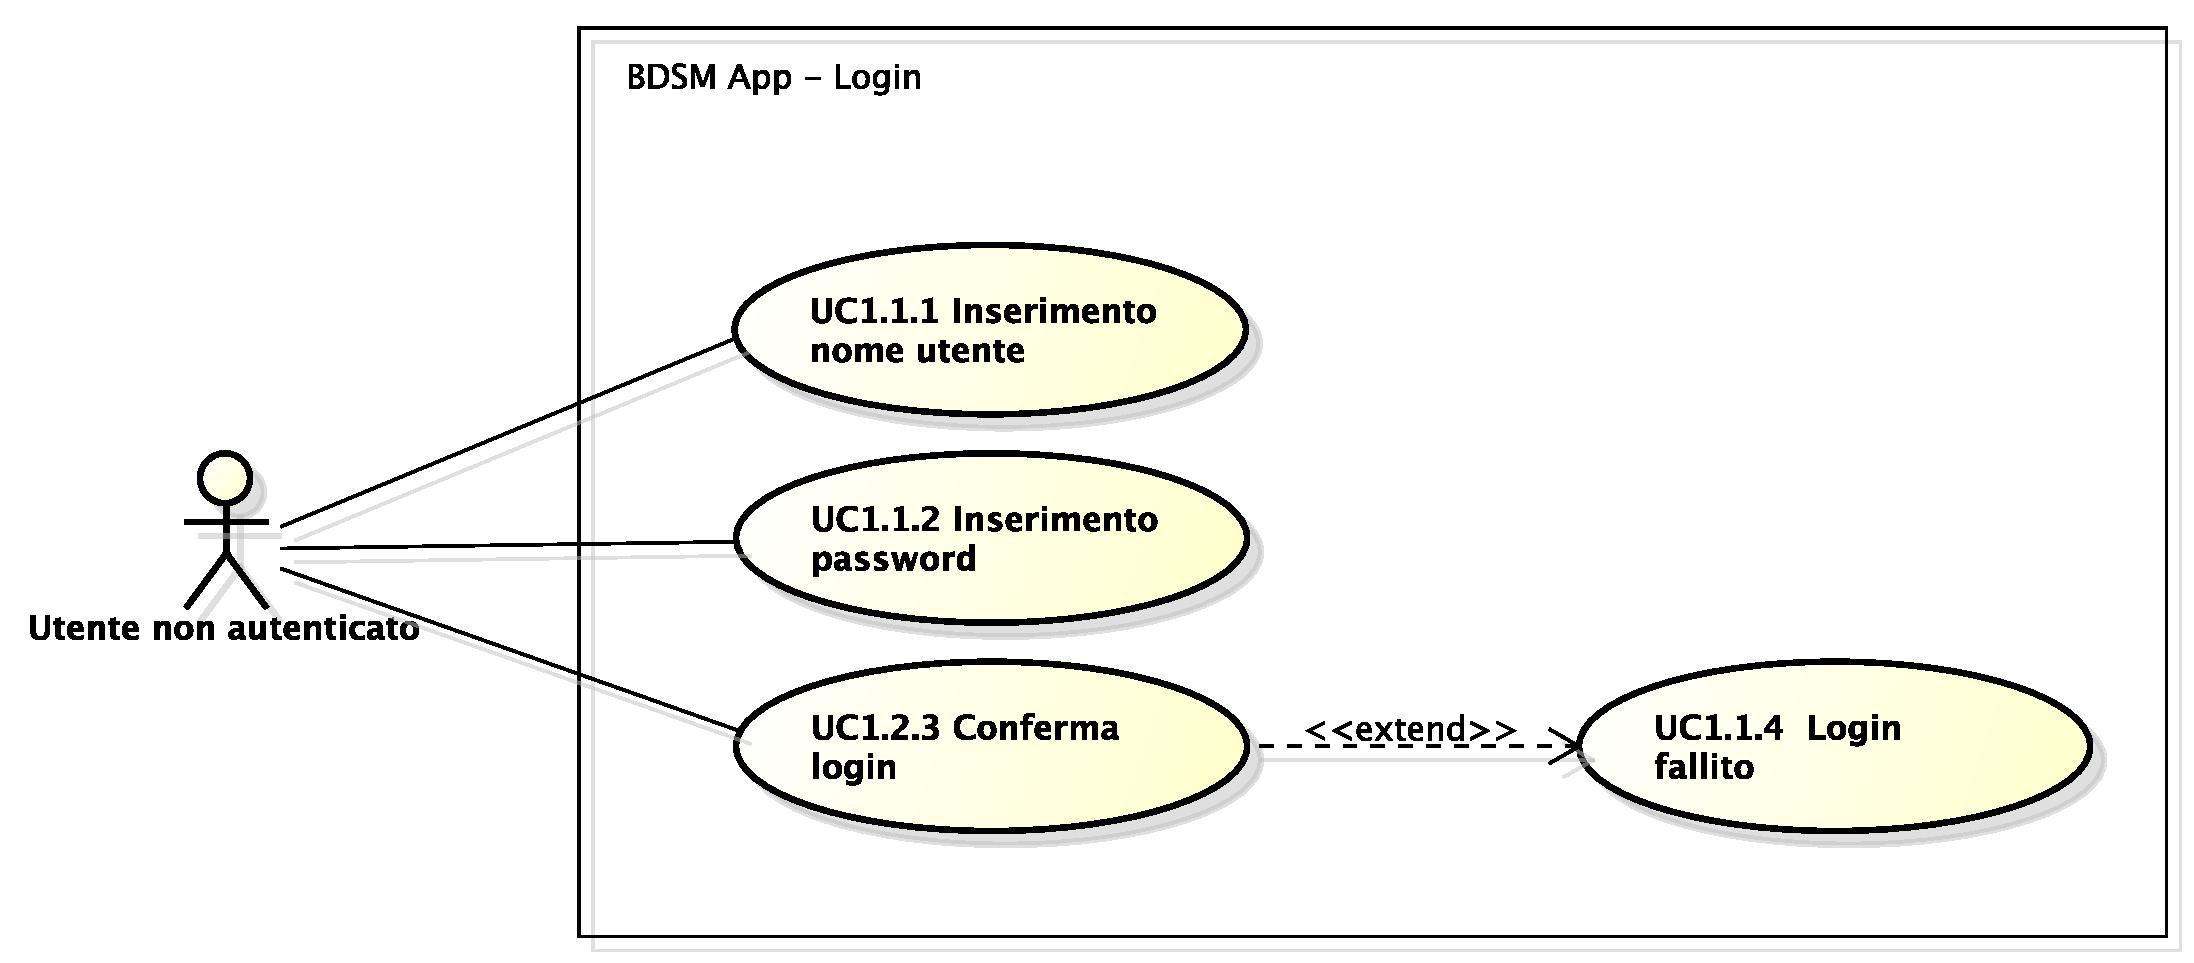
\includegraphics[scale=0.45]{./images/UC1_1.pdf}}
			\caption{D1 - Diagramma delle attività principali dell'utente non autenticato}
		\end{figure}
		[TO DO] (descrizione generale e elenco delle attività principali)

		% subsubsection attività_principali_dell_utente_non_autenticato (end)

		\subsubsection{D1.1: Registrazione al sistema} % (fold)
		\label{ssub:registrazione_al_sistema}
		\begin{figure}[!htbp]
			\centering
			\centerline{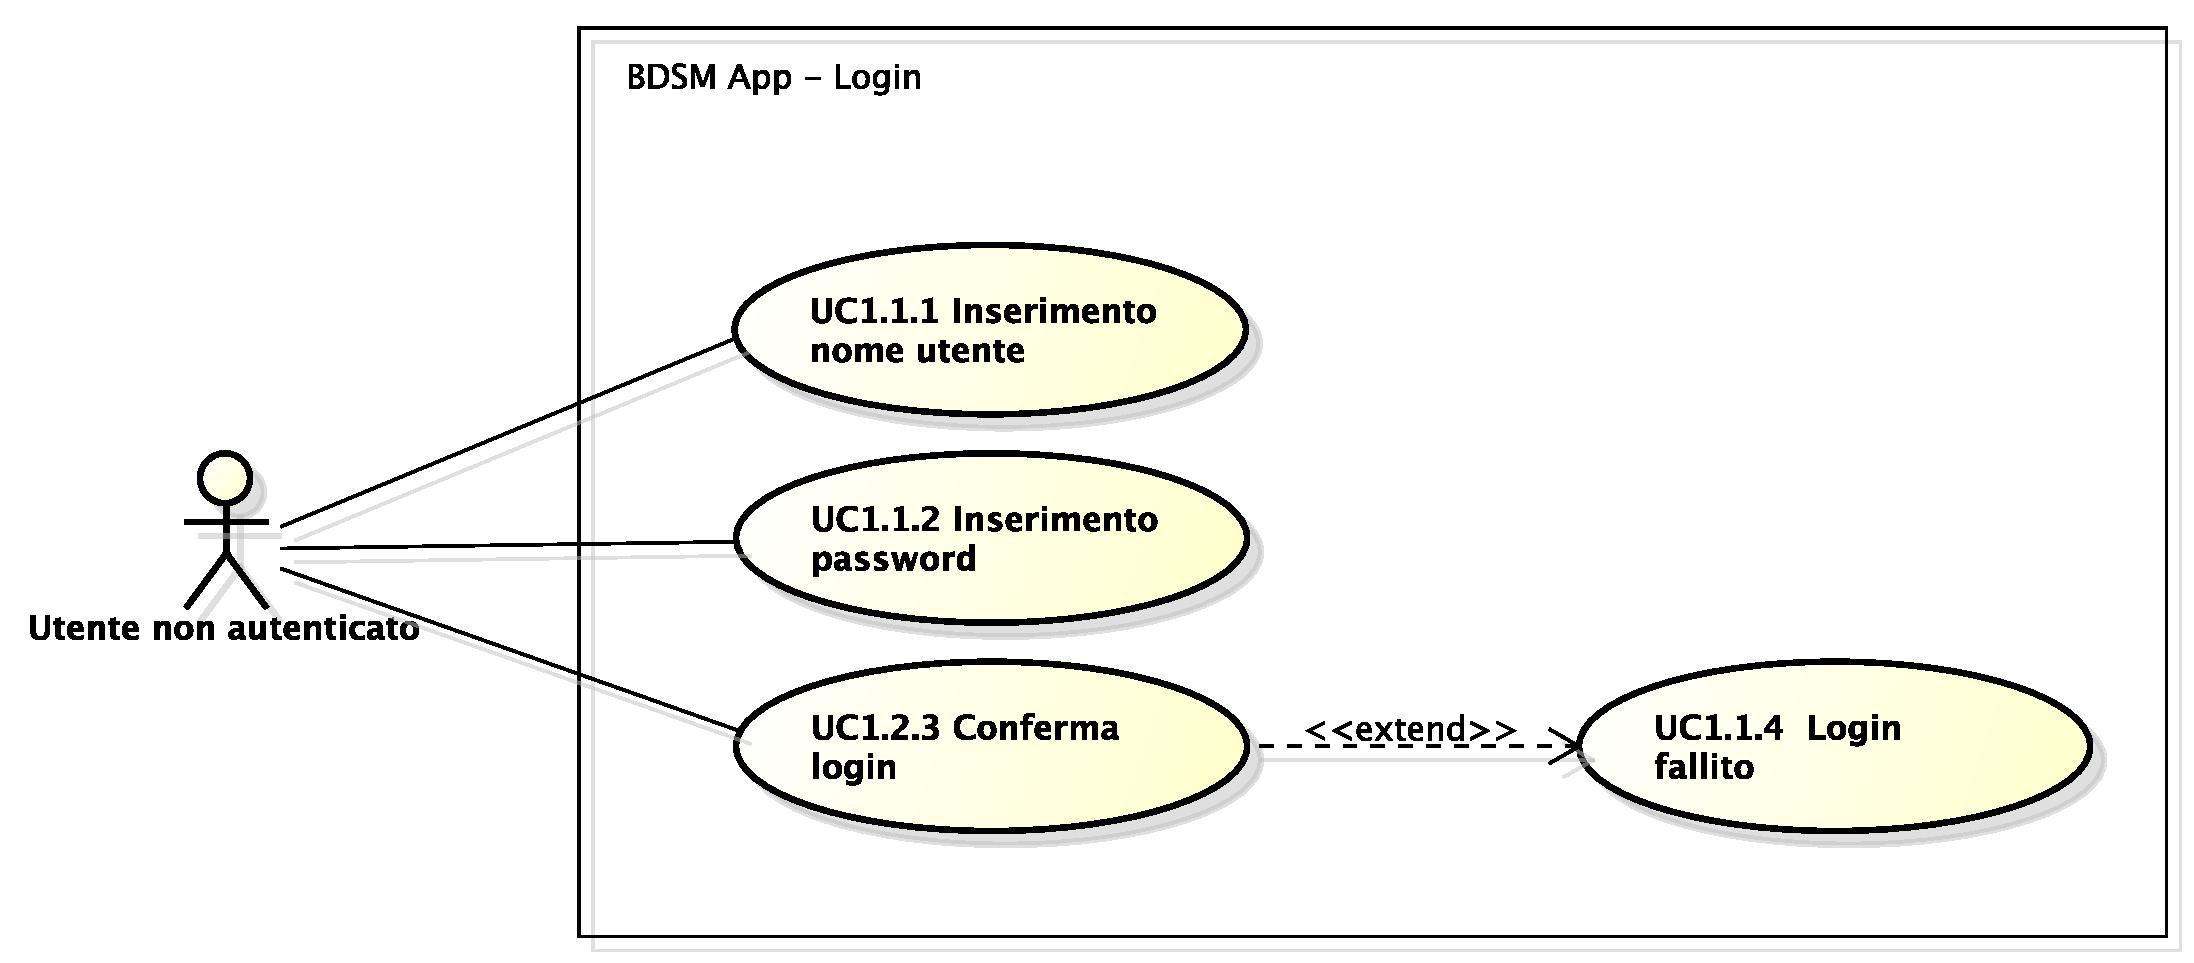
\includegraphics[scale=0.45]{./images/UC1_1.pdf}}
			\caption{D1.1 - Diagramma della registrazione al sistema}
		\end{figure}
		[TO DO] (descrizione generale)
		% subsubsection registrazione_al_sistema (end)

		\subsubsection{D1.2: Accesso al sistema} % (fold)
		\label{ssub:accesso_al_sistema}
		\begin{figure}[!htbp]
			\centering
			\centerline{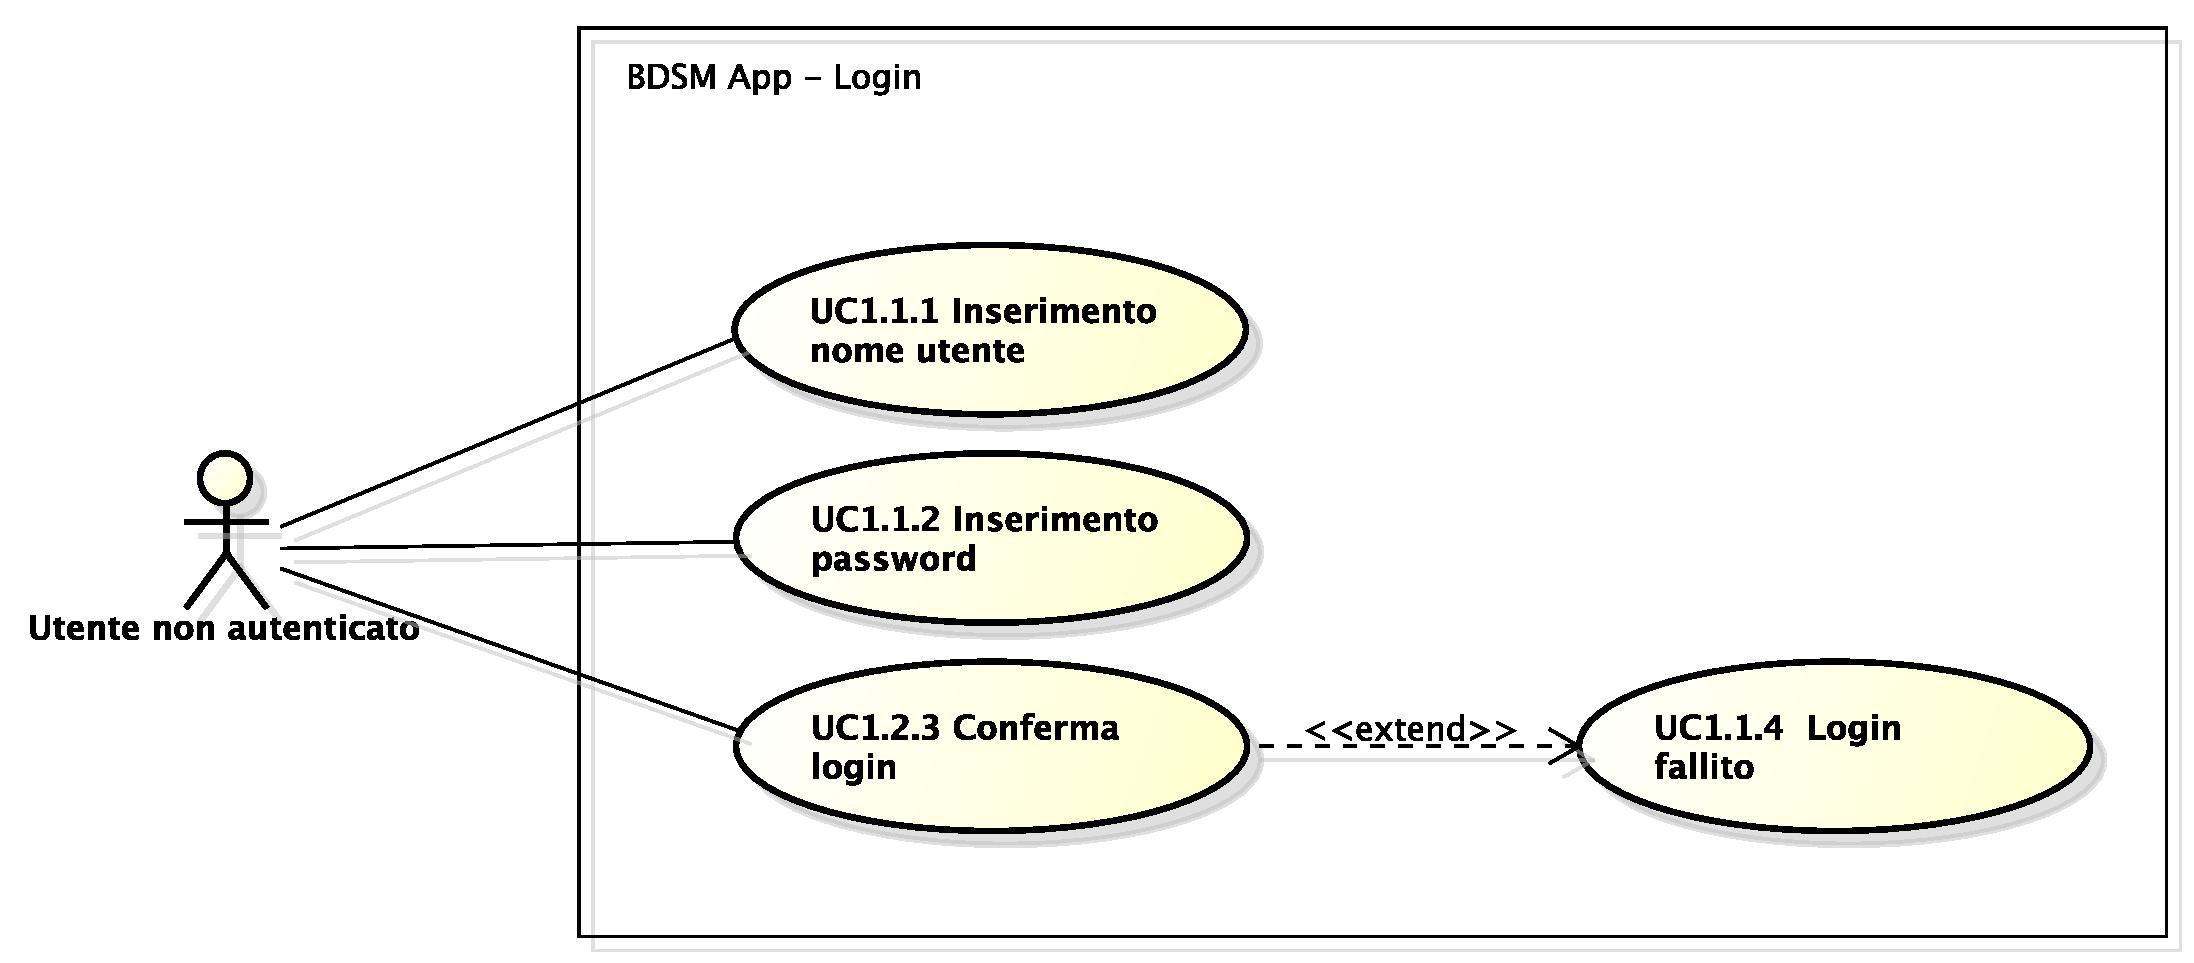
\includegraphics[scale=0.45]{./images/UC1_1.pdf}}
			\caption{D1.2 - Diagramma dell'accesso al sistema}
		\end{figure}
		[TO DO] (descrizione generale)
		% subsubsection accesso_al_sistema (end)

		\subsubsection{D1.3: Visualizzazione documentazione servizi REST} % (fold)
		\label{ssub:visualizzazione_documentazione_servizi_rest}
		\begin{figure}[!htbp]
			\centering
			\centerline{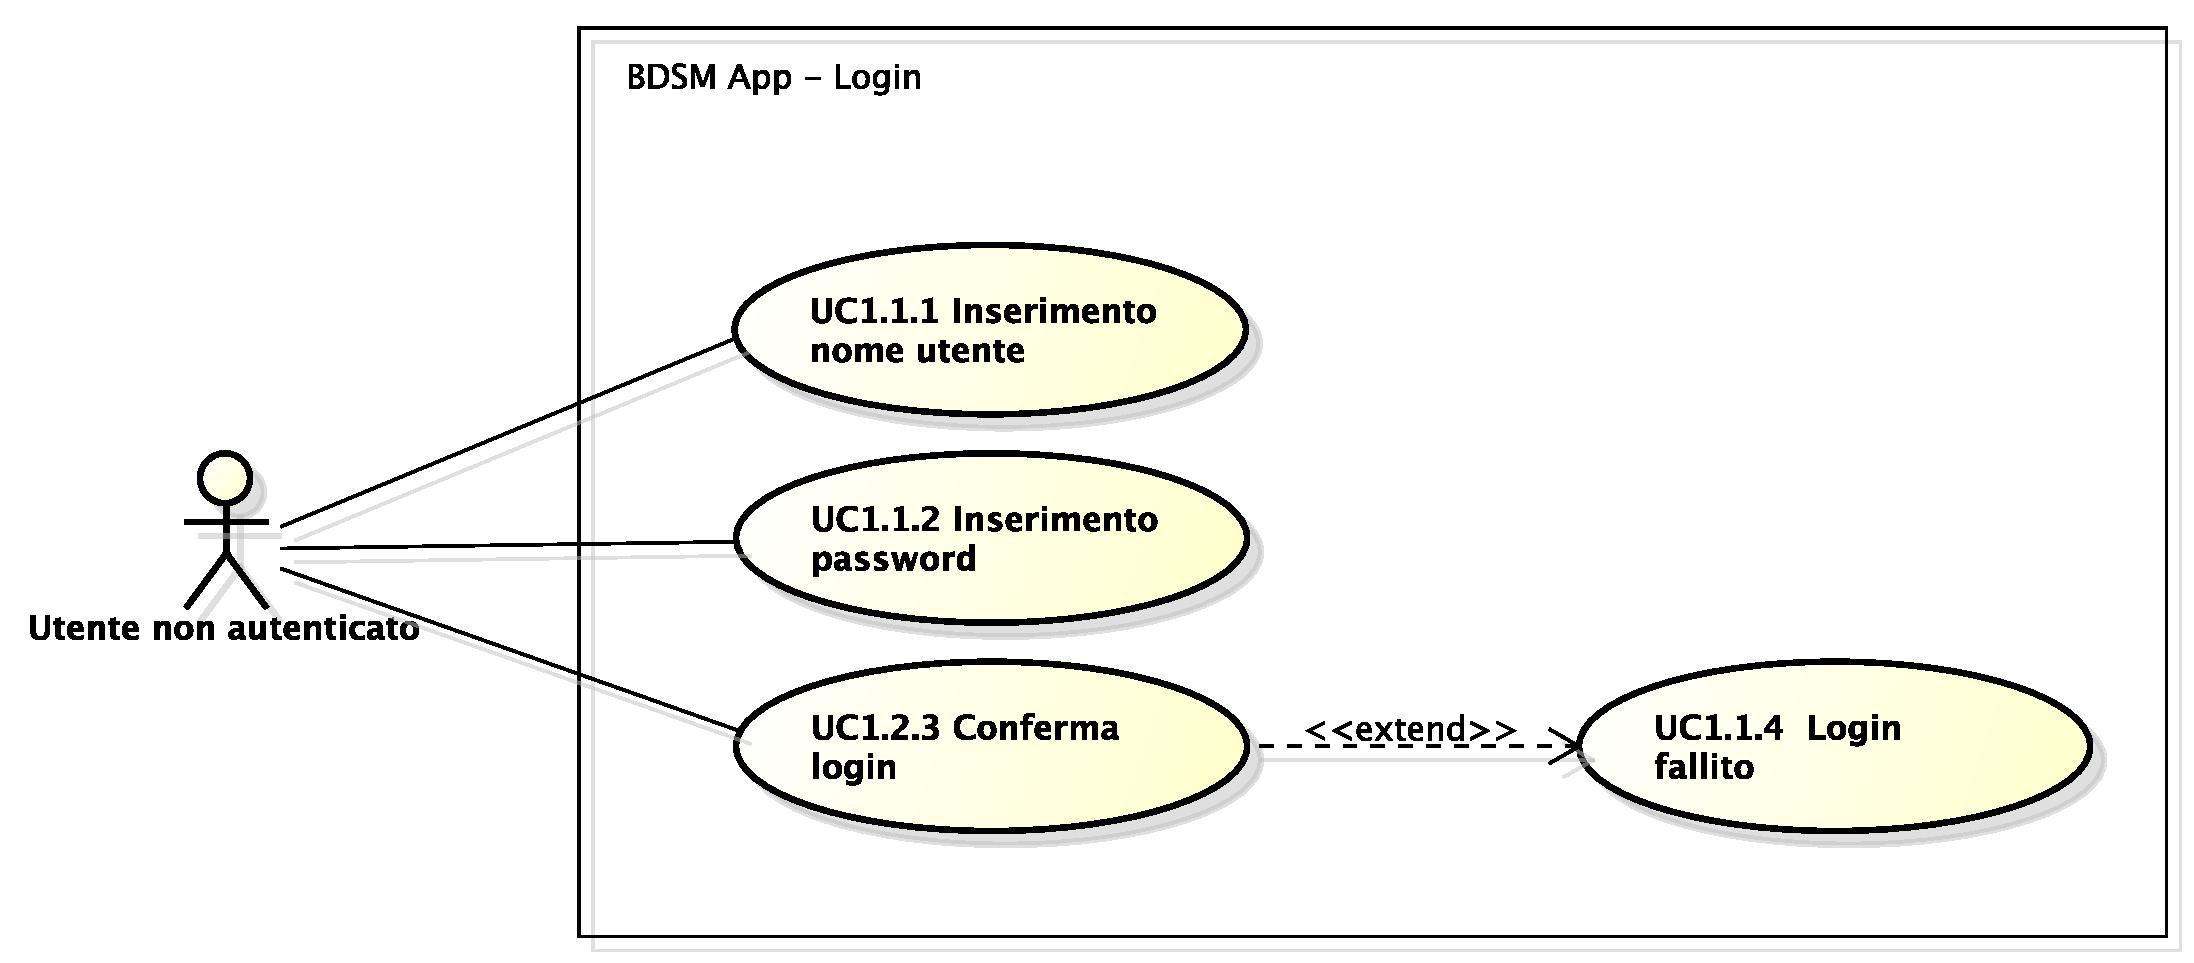
\includegraphics[scale=0.45]{./images/UC1_1.pdf}}
			\caption{D1.3 - Diagramma della visualizzazione documentazione servizi REST}
		\end{figure}
		[TO DO] (descrizione generale)
		% subsubsection visualizzazione_documentazione_servizi_rest (end)

	% subsection utente_non_autenticato (end)

	\pagebreak

	\subsection{Utente autenticato} % (fold)
	\label{sub:utente_autenticato}
	In questa sezione vengono illustrate le attività che un utente autenticato al sistema può compiere.
		\subsubsection{D2: Attività principali dell'utente autenticato} % (fold)
		\label{ssub:attivita_principali_dell_utente_autenticato}
		\begin{figure}[!htbp]
			\centering
			\centerline{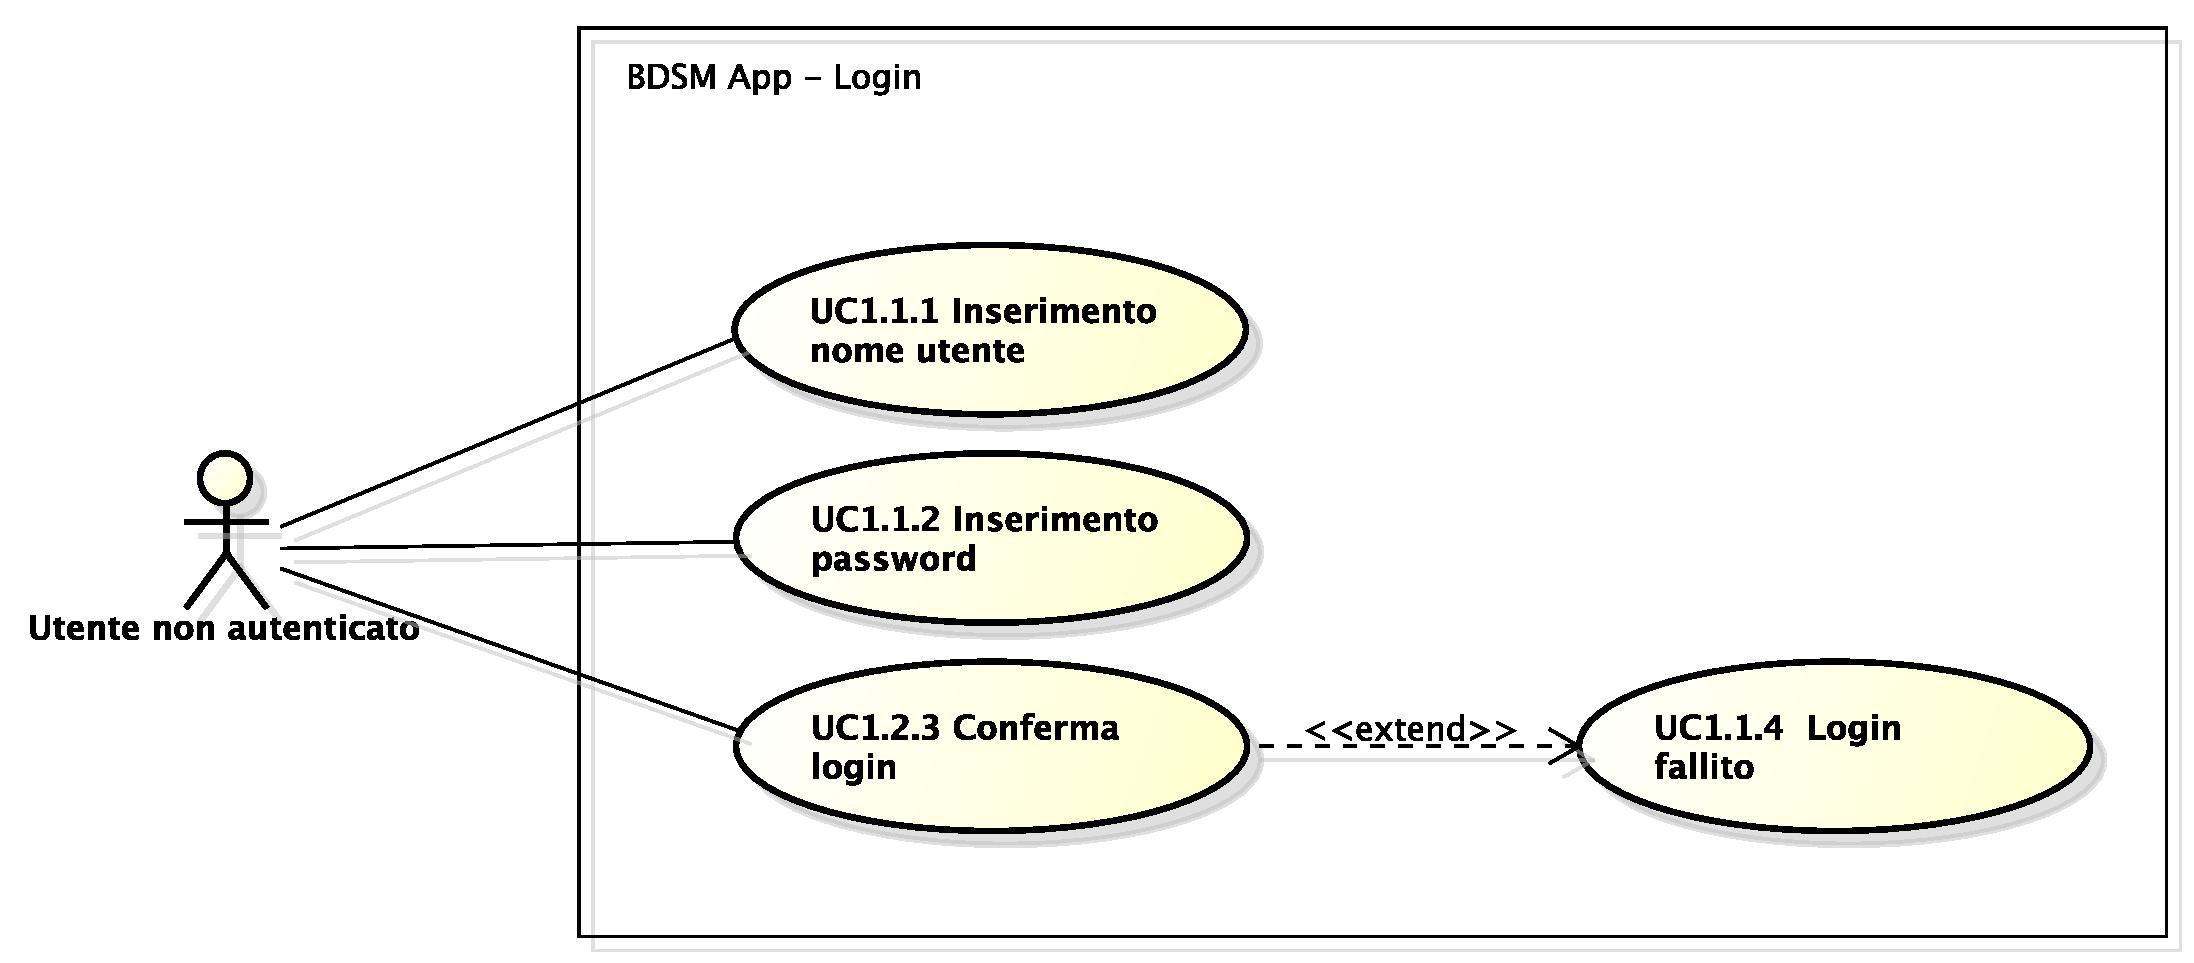
\includegraphics[scale=0.45]{./images/UC1_1.pdf}}
			\caption{D2 - Diagramma delle attività principali dell'utente autenticato}
		\end{figure}
		[TO DO] (descrizione generale e elenco delle attività principali)
		% subsubsection attività_principali_dell_utente_autenticato (end)


		\subsubsection{D2.1: Visualizzazione metriche di una Recipe} % (fold)
		\label{ssub:visualizzazione_metriche_di_una_recipe}
		[TO DO]
		% subsubsection visualizzazione_metriche_di_una_recipe (end)

		\subsubsection{D2.2: Confronto tra metriche di una Recipe} % (fold)
		\label{ssub:confronto_tra_metriche_di_una_recipe}
		[TO DO]
		% subsubsection confronto_tra_metriche_di_una_recipe (end)

		\subsubsection{D2.3: Visualizzazione dei preferiti} % (fold)
		\label{ssub:visualizzazione_dei_preferiti}
		[TO DO]
		% subsubsection visualizzazione_dei_preferiti (end)

		\subsubsection{D2.4: Richiesta di una nuova Recipe} % (fold)
		\label{ssub:richiesta_di_una_nuova_recipe}
		[TO DO]
		% subsubsection richiesta_di_una_nuova_recipe (end)

		\subsubsection{D2.5: Gestione token di accesso} % (fold)
		\label{ssub:gestione_token_di_accesso}
		[TO DO]
		% subsubsection gestione_token_di_accesso (end)

		\subsubsection{D2.6: Visualizzazione dettagli utente} % (fold)
		\label{ssub:visualizzazione_dettagli_utente}
		[TO DO]
		% subsubsection visualizzazione_dettagli_utente (end)

		\subsubsection{D2.7: Modifica dei dati utente} % (fold)
		\label{ssub:modifica_dei_dati_utente}
		[TO DO]
		% subsubsection modifica_dei_dati_utente (end)

		\subsubsection{D.7.1: Modifica della password} % (fold)
		\label{ssub:modifica_della_password}
		[TO DO]
		% subsubsection modifica_della_password (end)

	% subsection utente_autenticato (end)

	\pagebreak



	\subsection{Utente amministratore} % (fold)
	\label{sub:utente_amministratore}
	In questa sezione vengono illustrate le attività che un amministratore del sistema può compiere. L'utente amministratore oltre alle suddette potrà svolgere anche tutte le attività presenti nella sezione \ref{ssub:attivita_principali_dell_utente_autenticato}.
		\subsubsection{D3: Attività principali dell'utente amministratore} % (fold)
		\label{ssub:attivita_principali_dell_utente_amministratore}
		\begin{figure}[!htbp]
			\centering
			\centerline{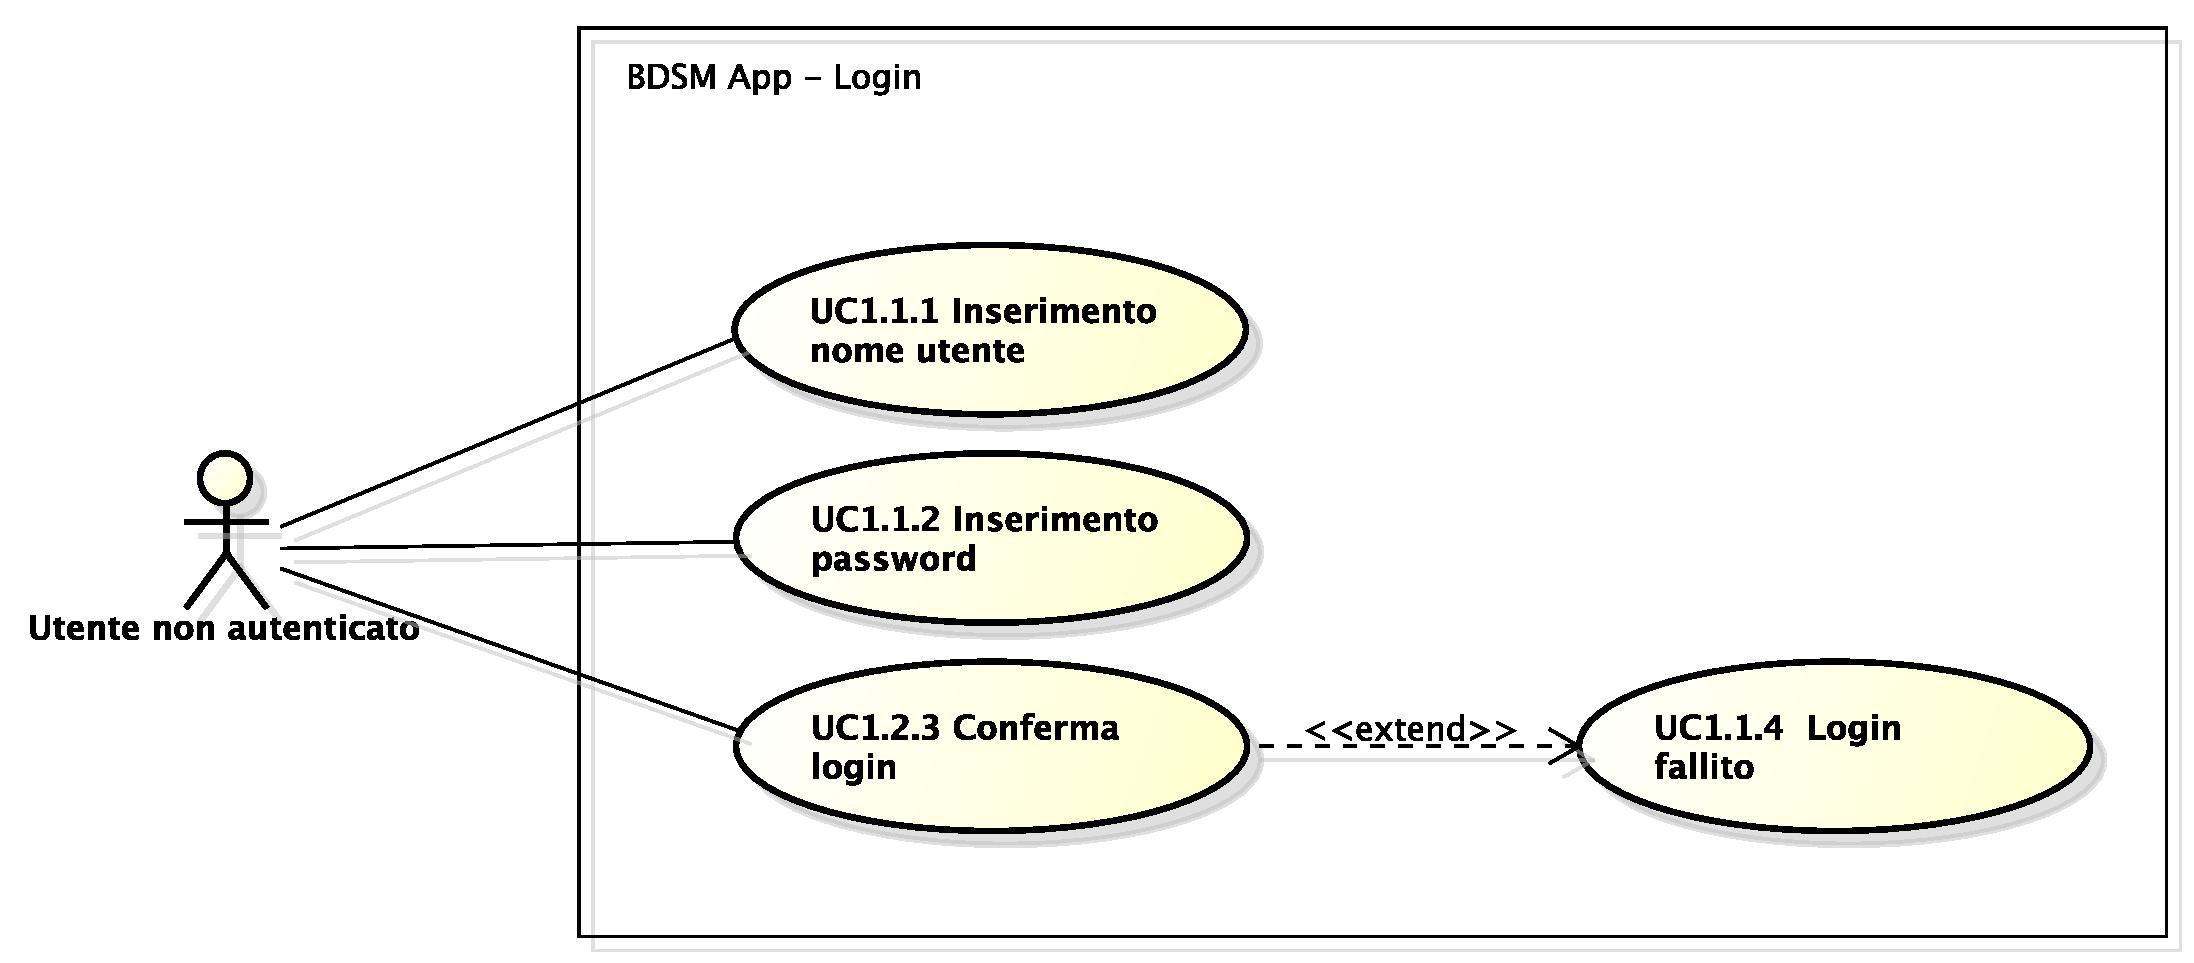
\includegraphics[scale=0.45]{./images/UC1_1.pdf}}
			\caption{D3 - Diagramma delle attività principali dell'utente amministratore}
		\end{figure}
		[TO DO] (descrizione generale e elenco delle attività principali)

		% subsubsection attività_principali_dell_utente_amministratore (end)


		\subsubsection{D3.1: Inserimento nuova Recipe} % (fold)
		\label{ssub:inserimento_nuova_recipe}
		[TO DO]
		% subsubsection inserimento_nuova_recipe (end)


		\subsubsection{D3.2: Gestione richieste Recipe} % (fold)
		\label{ssub:gestione_richieste_recipe}
		[TO DO]
		% subsubsection gestione_richieste_recipe (end)

		\subsubsection{D3.3: Amministrazione degli utenti} % (fold)
		\label{ssub:amministrazione_degli_utenti}
		[TO DO]
		% subsubsection amministrazione_degli_utenti (end)




	% subsection utente_amministratore (end)




% section diagrammi_delle_attività (end)